\documentclass{article}
\usepackage[utf8]{inputenc}
\usepackage[backend=biber]{biblatex}
\usepackage{amssymb}
\usepackage{amsmath}
\usepackage{dsfont}
\addbibresource{bib.bib}
\setlength{\parindent}{0em}
\bibliography{bib}
\setlength{\parskip}{6pt}
\usepackage[margin=1.0in]{geometry}
\usepackage{graphicx}
\usepackage{caption}
\usepackage{subcaption}
\usepackage{wrapfig}
\usepackage{url}

\title{Intro to deep learning with PyTorch}
\author{Miguel A. Saavedra-Ruiz}
\date{May 2020}
\linespread{1.0}

\nocite{*}


\begin{document}

\maketitle

\section*{Autoencoders}

The autoencoder is a very simple neural network and it is similar to the multi-layer perceptron. This network architecture is designed to reproduce its input at the output layer. The main differences between an Autoencoder and a MLP is that the number of input neurons is equal to the number of output neurons. 

\begin{figure}[ht]
    \centering
    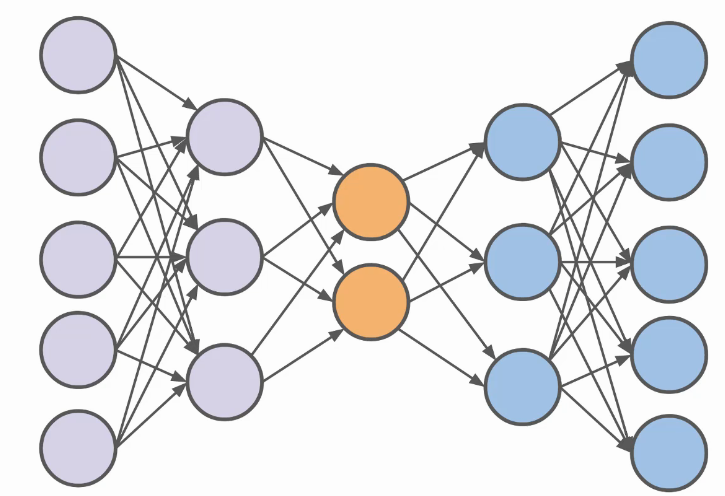
\includegraphics[width=0.35\textwidth,height=0.35\textheight,keepaspectratio]{images/auto.png}
    \captionsetup{justification=centering}
    \caption{Autoencoder with three hidden layers}
    \label{fig:f1}
\end{figure}

Fig. \ref{fig:f1} presents a simple stacked autoencoder with three hidden layers. As it is possible to see that the output size is the same as the input size. One important thing to note in that in the left size of the image the model starts with five input neurons and then then that gets reduced to three neurons in the first hidden layer and then to two in the second hidden layer. Subsequently, it gets gradually increased until the output layer has the same number of neurons as the input layer.

\begin{figure}[ht]
    \centering
    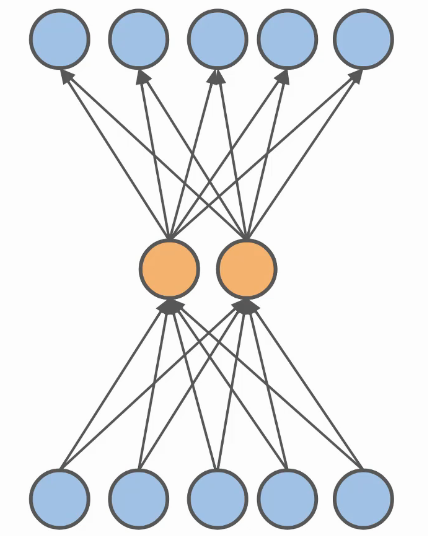
\includegraphics[width=0.25\textwidth,height=0.25\textheight,keepaspectratio]{images/simple_auto.png}
    \captionsetup{justification=centering}
    \caption{Autoencoder with one hidden layer}
    \label{fig:f2}
\end{figure}

To explain the basic idea behind an autoencoder let's use a simpler model presented in Fig. \ref{fig:f2}. This model basically has one hidden layer and then the output has the same dimension as the input layer. For the sake of notation, see Fig. \ref{fig:f3} which is another representation of the same model presented in Fig. \ref{fig:f2}. Recall that an autoencoder is a feedforward network that is trained to reproduce its input at the output. Therefore, what this network architecture is trying to do is directly mimic its input at the output layer.


As it is possible to notice, \(W\) are the weights between the input layer and the hidden layer, \(b\) is the bias term of the hidden layer and \(h(x)\) is the output of the hidden layer. Furthermore, \(W^{out}\) are the weights between the output layer and the hidden layer, \(c\) is the bias term of the output layer and \(\overline{x}\) is the output of the final layer Fig. \ref{fig:f3}. 

\begin{figure}[ht]
    \centering
    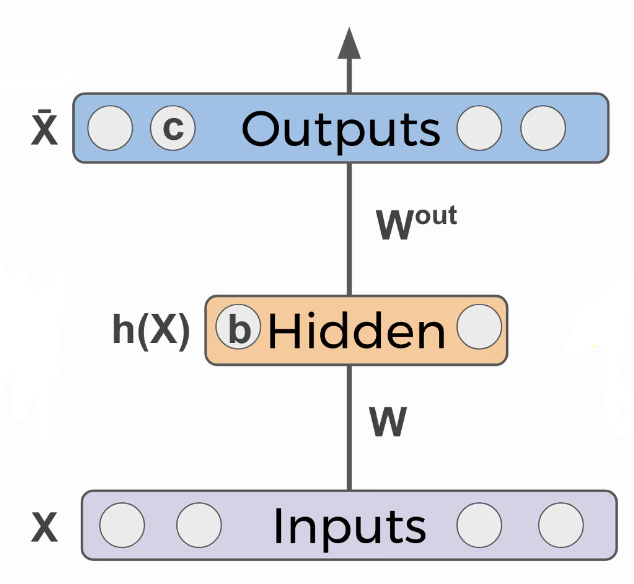
\includegraphics[width=0.35\textwidth,height=0.35\textheight,keepaspectratio]{images/architecture.png}
    \captionsetup{justification=centering}
    \caption{Representation of autoencoder with one hidden layer}
    \label{fig:f3}
\end{figure}

Mathematically, the equations for an autoencoer are exactly the same as the ones for an MLP. In this case, for the hidden layer the equation is given by \eqref{eq:2} and for the output layer is \eqref{eq:2}. There are two main parts in an Autoencoder and that is the first chunk of the autoencoder that goes from the input layer to the hidden layer (Encoder) and the second part which goes from the hidden layer to the output layer (Decoder). Hence, the encoder equation for the autoencoder presented in Fig. \ref{fig:f2} is given by \eqref{eq:1} and for the decoder by \eqref{eq:2}.

\begin{equation}
h(x) = \sigma(Wx + b)
\label{eq:1}
\end{equation}

\begin{equation}
\overline{x} = \sigma(W^{out}h(x) + c)
\label{eq:2}
\end{equation}

The main function of the encoder section is to find a compressed representation of the input layer. On the other hand, the function of the decoder is reproduce the input layer at the output. A really common practice with autoencoders is to use tied weights. This means that the weights coming from the input to the hidden layer are going to be the same weights between the hidden and output layer but transposed \(W^{out} = W^T\). This approach is possible owing to the autoencoder is basically train to reproduce the input at the output layer. It is important to mention that the only thing tied are the weights, the bias are not tied.

The key idea in an autoencoder is that the encoder section is trying to create an internal representation that maintains all the information of the input. The really important aspect about the encoder layer is that it is possible to use it to extract meaningful features from the input data and create a compressed representation. Owing to this benefit of the encoder, Autoencoders have been used for principal components analysis (PCA).

An Stacked autoencoder is the one presented in Fig. \ref{fig:f1} and it basically has more hidden layers and a bigger ability for abstraction.

One example of a simple autoencoder is presented in the code \textit{Simple\_Autoencoder.ipynb}. This code receives as input the MNIST dataset and the idea is to output the same input digit. This simple autoencoder architecture is presented in Fig. \ref{fig:f4}

\begin{figure}[ht]
    \centering
    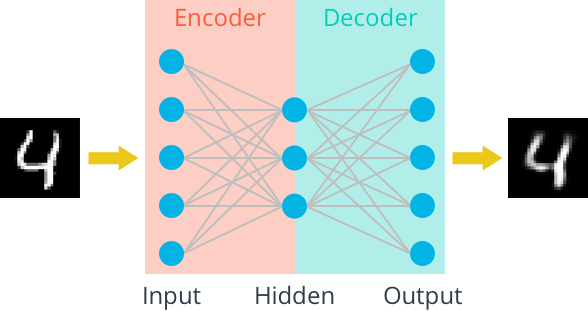
\includegraphics[width=0.45\textwidth,height=0.45\textheight,keepaspectratio]{images/simple_autoencoder.png}
    \captionsetup{justification=centering}
    \caption{Simple autoencoder example}
    \label{fig:f4}
\end{figure}

To understand the decoder phase in a convolutional neural network, it is necessary to introduce two additional concepts which make possible the generation of an output image of the same size of the input image. Let's first talk about \textbf{Upsampling}. This technique is basically defined as the opposite of Downsampling and the idea is increase the dimensions of the future map whereas the downsampling method reduce its dimensions. 

There are different techniques for upsampling. The first technique is called \textbf{Nearest Neighbors} and is presented in Fig. \ref{fig:f5}. As the name suggests it takes an input pixel value and copy it to the K-Nearest Neighbors where K depends on the expected output.

\begin{figure}[ht]
    \centering
    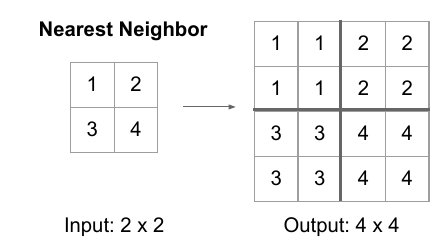
\includegraphics[width=0.45\textwidth,height=0.45\textheight,keepaspectratio]{images/nn.png}
    \captionsetup{justification=centering}
    \caption{Nearest Neighbors (Upsampling)}
    \label{fig:f5}
\end{figure}

\textbf{Bed Of Nails} is other upsampling technique where the value of the input pixel is copyed at the corresponding position in the output image and filling zeros in the remaining positions Fig. \ref{fig:f6}.

\begin{figure}[ht]
    \centering
    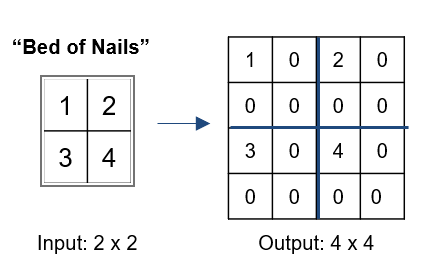
\includegraphics[width=0.45\textwidth,height=0.45\textheight,keepaspectratio]{images/bn.png}
    \captionsetup{justification=centering}
    \caption{Bed of Nails (Upsampling)}
    \label{fig:f6}
\end{figure}

Finally, \textbf{Max-Unpooling} which basically takes the maximum among all the values in the kernel. This process is performed by saving the index of the maximum value for every max-pooling layer during the encoding step. The saved index is then used during the Decoding step where the input pixel is mapped to the saved index, filling zeros everywhere else.

\begin{figure}[ht]
    \centering
    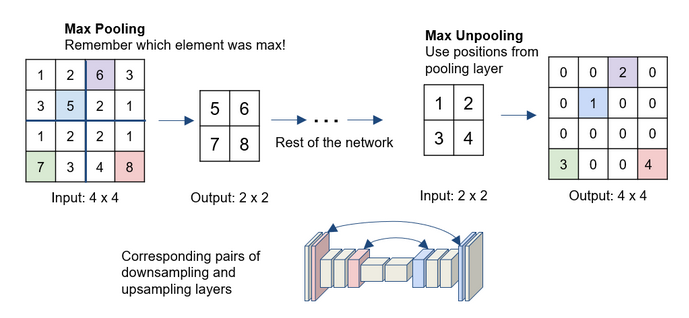
\includegraphics[width=0.85\textwidth,height=0.85\textheight,keepaspectratio]{images/mn.png}
    \captionsetup{justification=centering}
    \caption{Max-Unpooling (Upsampling)}
    \label{fig:f6}
\end{figure}

Besides upsampling, there is another popular method used to increase the dimensions of the feature map and this is called \textbf{Trasposed convolution}. This method is widely used and has multiple applications in super image resolution and image segmentation. Usually this method is preferred over upsampling. A Transposed convolution takes an input feature map to generate an output feature map which has a spatial dimension greater than that of the input feature map. This technique uses a kernel whose values are learned during the training procedure.

The transposed convolution has the same parameters as a convolutional layer. The Stride, Padding and kernel size are exactly the same. Nevertheless, it is necessary to introduce new parameters for this process. The first parameter is \(z\) and is defined as the amount of zeros between pixel in the feature map Eq. \eqref{eq:3}, the second parameter is \(p'\) which is the new padding to use in the input feature map Eq. \eqref{eq:4}. The stride in a transposed convolutional layer is defined as \(s' = 1\) and this is always one. It is important to recall that \(k\) is the filter size.

\begin{equation}
z = s - 1
\label{eq:3}
\end{equation}

\begin{equation}
p' = k - p - 1
\label{eq:4}
\end{equation}

The steps to perform a transposed convolution are given as follows:

\begin{itemize}
  \item Calulate new parameters \(z\) and \(p'\)
  \item Between each rows and columns of the input, insert \(z\) number of zeros. This increases the size of the input to \((2*i-1),(2*i-1)\)
  \item Pad the modified input image with \(p'\) number of zeros
  \item Carry out standard convolution on the image generated from step 3 with a stride length of 1
\end{itemize}

In the Fig. \ref{fig:f7} are given the steps mentioned above. 

\begin{figure}[ht]
    \centering
    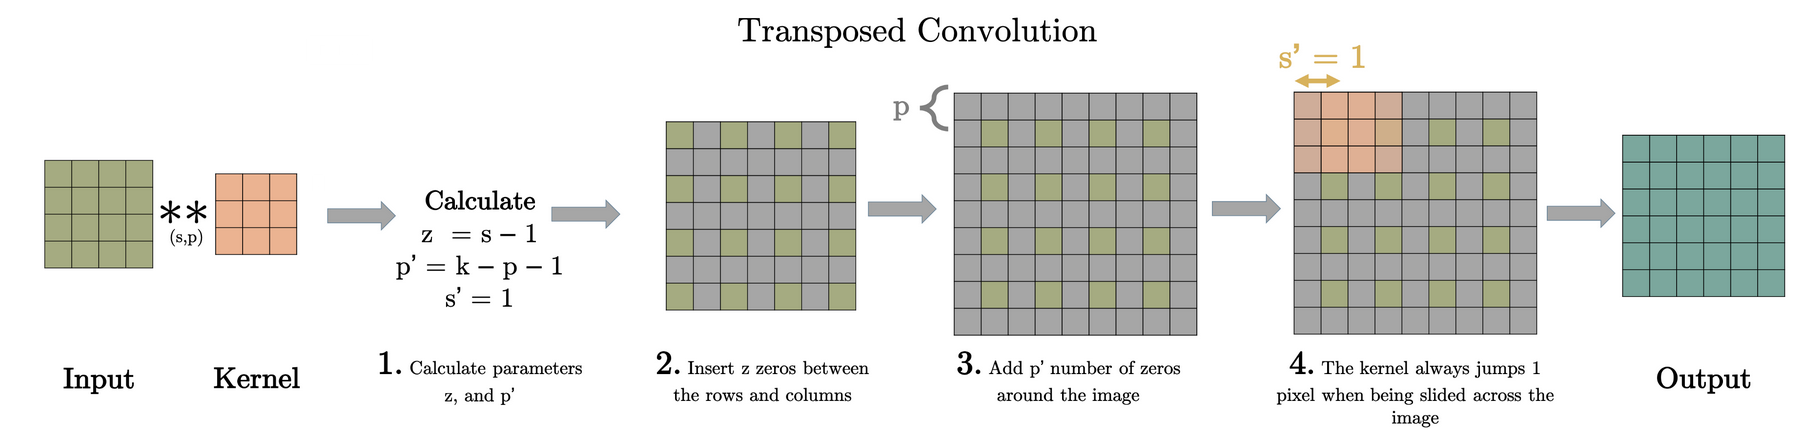
\includegraphics[width=0.95\textwidth,height=0.95\textheight,keepaspectratio]{images/transposed_conv.png}
    \captionsetup{justification=centering}
    \caption{Transposed convolution}
    \label{fig:f7}
\end{figure}

Additionally, Fig. \ref{fig:f8} presents examples of transposed convolutions with different stride and padding.

\begin{figure}[ht]
    \centering
    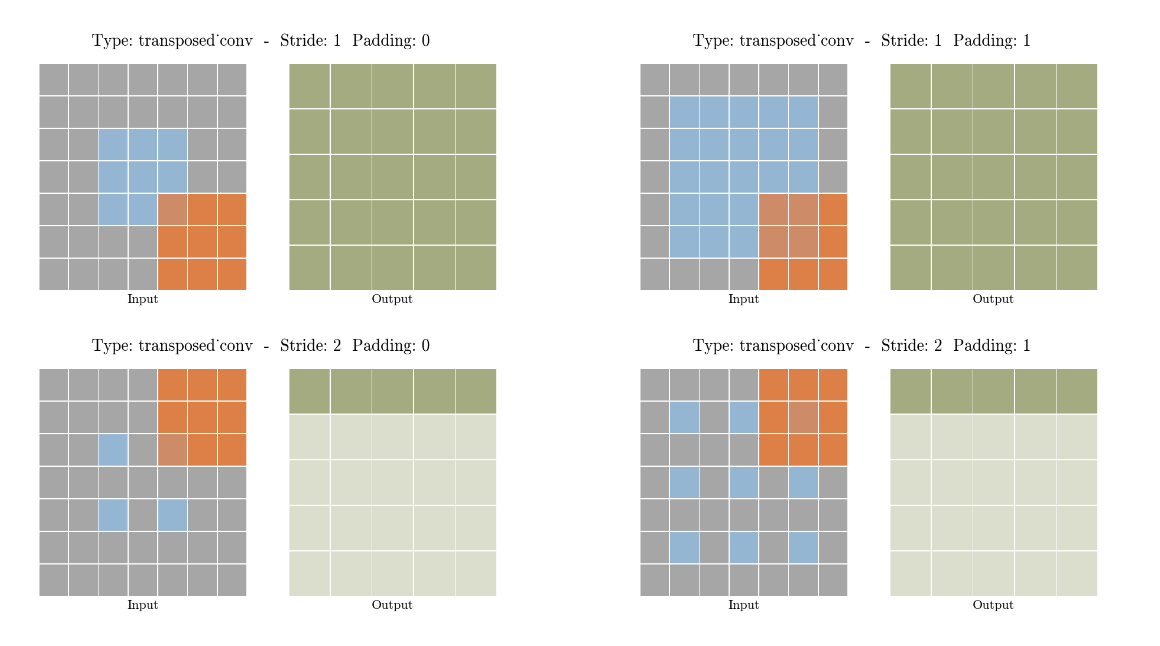
\includegraphics[width=0.95\textwidth,height=0.95\textheight,keepaspectratio]{images/multiple_convs.png}
    \captionsetup{justification=centering}
    \caption{Transposed convolution examples}
    \label{fig:f8}
\end{figure}

For a given size of input (\(i\)), kernel (\(k\)), padding (\(p\)) and stride (\(s\)), the size of the output feature map (\(o\)) generated is given by  Eq. \eqref{eq:5}.

\begin{equation}
o = (i - 1) * s + k - 2p
\label{eq:5}
\end{equation}

A implementation of a denoising autoencoder with CNNs can be seen at \textit{Denoising\_Autoencoder\_Exercise.ipynb}. This file receives a noisy MNIST image and the neural network is able to reconstruct the image without noise. The main idea behind a denoising autoencoder is that the network is trained with noisy data and the output is the data without nouse. This is one of the biggest application of autoencoders and as they are able to create a compressed representation of the data, they are very good at reconstructing the data without noise.

Another adventage of autoencoders of autoencoders is that they learn a pretty descent representation of the weights of the a network just with the input. The autoencoders can be used as a initializer and then use the learned weights as the initial ones for a fine-tuning process. This kind of approach have shown good results and ease the training procedure of neural networks.

\printbibliography


\end{document}
